\documentclass{article} % For LaTeX2e
\usepackage{nips13submit_e,times}
\usepackage{hyperref}
\usepackage{url}
\usepackage{graphicx}
\usepackage{alltt}
\renewcommand{\ttdefault}{txtt}




\title{Color Detection Under Supervised Learning}

\author{
Cyrus Anderson \\
University of Michigan \\
\texttt{andersct@umich.edu} \\
\And
Jocelyn Bohr \\
University of Michigan \\
\texttt{bjocelyn@umich.edu} \\
\AND
Michael Lu \\
University of Michigan \\
\texttt{lumike@umich.edu} \\
\And
Nghia Vo \\
University of Michigan \\
\texttt{thnghia@umich.edu} \\
}

% The \author macro works with any number of authors. There are two commands
% used to separate the names and addresses of multiple authors: \And and \AND.
%
% Using \And between authors leaves it to \LaTeX{} to determine where to break
% the lines. Using \AND forces a linebreak at that point. So, if \LaTeX{}
% puts 3 of 4 authors names on the first line, and the last on the second
% line, try using \AND instead of \And before the third author name.

\newcommand{\fix}{\marginpar{FIX}}
\newcommand{\new}{\marginpar{NEW}}

\nipsfinalcopy % Uncomment for camera-ready version

\begin{document}

\maketitle

\begin{abstract}
In this report, we present multiple supervised learning approaches to a common problem: color classification. From the simple k-nearest neighbors to machine learning SVM, there are a variety of approaches to this problem. Some solutions may perform better than others depending on the specific application and constraints. Here, our objective is to classify the colors of buoys on the surface of a pond during an autonomous robotic boat challenge under various conditions (e.g. time of day, weather, and lighting conditions). Our aim is to allow the autonomous robotic boat to use our classifier to make color classifications during the challenge. This report will compare results from basic non-learning algorithms such as majority-voting and average color, with more sophisticated learning algorithms such as multiclass SVM with linear and RBF kernel, Naive Bayes, and Softmax Regression. This report also details how we use a 3D modeling software to generate synthetic training images of buoys under all lighting conditions to further improve test accuracy. 
\end{abstract}

\section{Introduction}
Each summer, the autonomous robotic boat team UM:Autonomy at the University of Michigan competes in the Association for Unmanned Vehicle Systems International's RoboBoat competition held in Virginia Beach, Virginia against various other robotics labs and clubs. Since a pond serves as the site for the various challenges used to judge the robots, buoys act as the primary landmarks. However there are often few other objects used as landmarks. Buoys often serve as the source of loop closures in the robot's long term path planning, allowing the robot to build an accurate internal map and minimize drift. Knowing additional features such as color can reduce contradictory information that produce incorrect mapping. Buoys also serve as boundaries or goals for certain challenges [2]. For example, some challenges involve determining the buoy color. Thus there is substantial need to accurately identify buoy color.
\\\\Currently, the UM:Autonomy robotic boat relies on color filters to determine color. The process involves specifying bounds in RGB values for each color of buoy, then classifying buoys according to their match with the closest color template. These filters are faulty because the tuning is highly susceptible to be biased towards current lighting conditions, which results in detections that work well for several hours before deteriorating in accuracy. This is especially apparent in Virginia where the sun will be high in the sky (casting glare on the buoys and water) for most of the day with the occasional cloud passing in front to cast a shadow on the entire competition ground. Rainy and overcast days present another set of lighting conditions. Even on days when the sun stays high in the sky, backlit green buoys can appear black \textit{(fig.1 left)}, yellow can appear green, and washed out red may look orange. Additionally, white and black are difficult to filter since the filters for these colors generally have high false positive rates and end up including the very light or very dark patches of water produced with the 
noon sun's lighting \textit{(fig.1 right)}.
\\\\In this paper, we examine the results of various supervised learning techniques applied to classifying buoy color and aim to create a procedure to accurately classify buoy colors in a variety of lighting conditions. We attempt to create a robust system that runs faster than the cameras' frame rate of 10 Hz while leaving sufficient resources for the boat's other processes.


\begin{figure}[h]
\begin{center}
%\framebox[4.0in]{$\;$}
\fbox{\rule[0cm]{0cm}{0cm} 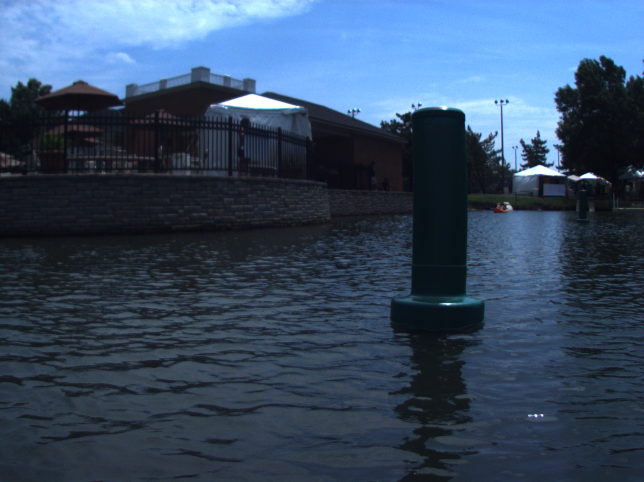
\includegraphics[scale=0.2]{difficult_green}
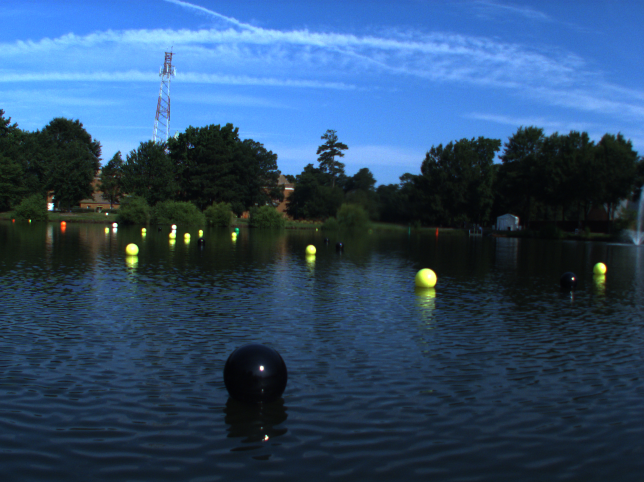
\includegraphics[scale=0.2]{difficult_black}
 \rule[0cm]{0cm}{0cm}}
\end{center}
\caption{Difficult buoys}
\end{figure}


\section{Proposed Method}

\subsection{Preprocessing}
The robotic boat has two Point Grey Flea 2, 1.3 MP %necessary to include the camera type?
cameras that publish images over the robot's Lightweight 
Communications and Marshalling (LCM) framework at 10 Hz. Logging utilities use LCM to capture and store various messages. Then the datasets are crafted from the different logs of the robot's runs. We label each boat photo by hand: marking the color and rectangle around each buoy within about 30 feet from the boat. From each rectangle, we extract the associated color histogram into a $256 \times 256 \times 256$ feature vector; each entry represents the frequency of the RGB color associated with the entry index. We then reduce this feature vector to a vector of size $16 \times 16 \times 16$, to make feature vectors less sparse and to decrease the classification time (since we are building this for a real time application).

\begin{figure}[h]
\begin{center}
%\framebox[4.0in]{$\;$}
\fbox{\rule[0cm]{0cm}{0cm} 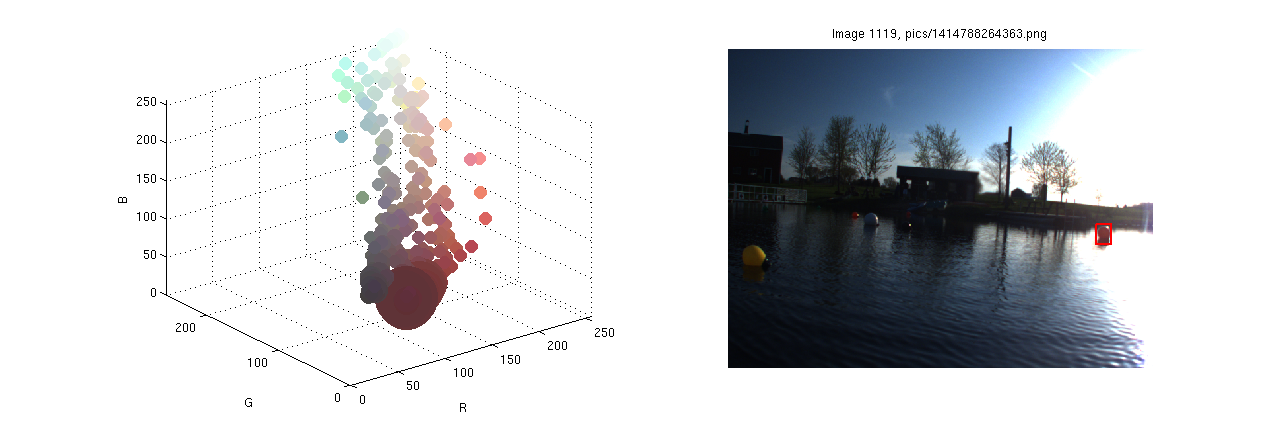
\includegraphics[scale=0.375]{visualization} \rule[0cm]{0cm}{0cm}}
\end{center}
\caption{Histogram visualization with labelled red buoy}
\end{figure}
% todo: pixel based/channel based preprocessing explanation, with photos

\subsection{Synthetic Data}
% maybe synthetic data fits here?? include photos of synthetic data

\subsection{Classification}
In this project, we compare classification results from multiclass SVM with linear and RBF kernel, multinomial Naive Bayes, and Softmax Regression. Our data set includes 2075 hand labeled real buoys under varied lighting conditions (cloudy, sunny, shady, etc) distributed amongst the 6 different colors, red, blue, black, green, yellow, and white. To support the real data, we also generated 8415 synthetic buoys under all lighting conditions. We divide the real data into 5 blocks of equal size, ensuring each block contains buoys under varied lighting conditions, and that the test set and training set are temporally different. We validate and test on exclusively real data, because our aim is to optimize a model for the real application. We also want to classify buoys faster than the  boat captures them (10 Hz). Because each photo has around 4 buoys, we need to classify each buoy faster than 0.025 seconds.\\\\
We began with SVM because it is a parametric algorithm; we do not need to store entire training data set to make predictions on the boat. It is also kernelized, which provides us with the flexibility to create arbitrarily complex boundaries. SVM prediction can be used to calculate confidence values for the decision by taking the distance from the separating hyperplane, which can be a useful measurement. SVM does not make any assumptions about the underlying distribution of the data. It is a widely used classification algorithm, so it can appropriately serve as our baseline classification algorithm. We used LIBSVM for our SVM classification, which utilizes a one-vs-rest multi-class classification scheme. We build SVM models with both linear and RBF kernel, and use 4-fold cross validation to appropriately select hyperparameters. With RBF kernel, each classification takes 0.0414 seconds per buoy, and with linear kernel each classification takes 0.0433 seconds per buoy. This may be slower than classification time for the real application because the these tests we run on CAEN's SSH servers, which may limit user resources.\\\\
We also used Naive Bayes because it has a simple implementation and it performs well even on small sets of training data. Naive Bayes is also parametric; we do not need to store the entire training data set to make decisions during the real time application. A parametric classifier is essential, since it is impractical to store all training data on the boat to make decisions in real time. Naive Bayes is also fast in training and testing, which is ideal for this application. The multinomial Naive Bayes classifier works well for classification with discrete features, such as color frequencies of pixels in a certain section of a photo, or word frequencies of a text document (e.g. the classic spam application). We utilized MATLAB's multinomial Naive Bayes classifier. Each classification takes 0.0012 seconds per buoy.\\\\
% todo: softmax regression (michael?) takes 0.00067 seconds per buoy

\section{Related Work}
% i think cyrus adds more related work?

The main set of approaches to this problem may be classified under pixel based segmentation; representative areas based on pixels from each image are categorized using predetermined classes of color, and the resulting information is used to classify the entire object's color [1b]. This set broadly includes histogram methods, clustering in the color space, and fuzzy clustering. Histogram methods first create histograms of colors split into different bins by their different coordinates, and then classify using intervals about peaks in the histograms [1c, 1d, 1e]. Clustering examines the distance between pixels in a given color space and assigns each pixel to its closest cluster [1f, 1g], whereupon the cluster characteristics such as center and size can be used for the object's classification. Fuzzy clustering first fuzzifies all pixels. This means assigning pixels such that each pixel is allowed to partially belong to multiple clusters. The assignment to these fuzzy clusters is accomplished through a predetermined or learned membership function [1h, 1i]. Next the clusters are defuzzified to enable a strict classification of the object. Additionally, there is another strand of work that seeks to account for color introduced by the illuminant, called color constancy [1j, 5]. This most directly addresses the problem of transforming an arbitrarily illuminated image to one under a given illuminant. Outdoors, the usual illuminant is the Sun and the desired illuminant is white light. Applying a color constancy algorithm to the images before using a pixel based method could increase accuracy by setting all data to have the same illuminant. Since early formulations of color constancy algorithms [6], more recent versions have reduced complexity to that of a FFT [7].

Real time application requires that each image must be processed in less than a third of a second, corresponding to listening to a stream of images from a camera publishing at 10 Hz. This narrows the available options to the faster methods. This eliminates most color constancy methods which tend to be slow [1j], many segmentation algorithms [1a], and fuzzy methods. We are thus left with lightweight histogram and cluster-based methods, which are simpler, easier to implement, and easier to interpret than fuzzy clustering. Color histograms have been in use for some time since their introduction [8] and are popular due to their invariance to translation and rotation in viewing perspective, and their robustness under changes in viewing angle and scale. The low computational complexity of color histograms makes them ideal for fast paced environments unsuitable for many more complex color detection techniques from computer vision. Furthermore, color histograms have been successfully applied to robotic soccer [3] and other realtime applications [4, 9].

In order to compare results to other algorithms suited for real time application, we looked for state-of-the-art algorithms but found none specific to this problem. Among those that were adaptable, all were difficult to implement. We thus implemented majority vote and average vote to classify the buoy colors, because it seemse reasonable to assume the most common or average pixel color within the buoy boundary can be representative of the buoy color. Both algorithms achieve low accuracies, but are better than randomly guessing a color.

\subsection{Majority vote}
Begin by iterating over the feature vector (described earlier in preprocessing), and choose the index with the highest count. Then compute the RGB vector by converting the index in the feature vector to the index in the original histogram, and store it as the most popular color. Compute the Euclidean distance between this RGB vector and the RGB vectors of our 6 colors, and classify the associated buoy as the color which yields the smallest distance.\\
The result was not as high as we expected, as many of the non-black buoys were classified as black because the shadow and water surface included in the picture popularized the count of black/near-black colors in the feature vector. The accuracy for majority vote over our real data set is 33.5\%.

\subsection{Average vote}
Begin by iterating over all the RGB values, then construct an RGB vector representing the total weighted sum of the RGB counts in the feature vector. Find the average RGB value by dividing by the total counts in the feature vector. Compute the Euclidean distance between this RGB vector and the RGB vectors of our 6 colors and classify the associated buoy as the color which yields the smallest distance.\\
The accuracy for average vote over our real data set is 35.7\%. This can again be attributed to the mixture of background in the picture boxes and also light variation across the buoys.

\section{Experimental Results}

% todo: charts for train/test accuracies, change this explanation
% include photos for misclassified buoys
Using both linear SVM and multinomial Naive Bayes, we achieve high accuracy rates (compared to baseline methods discussed in related works). With a sufficient number of training examples, both methods achieve over 98\% accuracy. Naive Bayes performs marginally better, and the advantage of Naive Bayes is emphasized when fewer training examples are used. Each average accuracy is calculated by selecting a random training set of size $n$, then selecting a random testing set of size 130 from the remaining data, and finally train and test classifiers accordingly. The average accuracy is taken over 10 classification results. Although these accuracies are high, we believe one contributing factor can be attributed to a fairly homogeneous data set. We do not have enough variation in our data set, so classification is easier. This problem, and how we intend to solve it, will be discussed in the future milestones section. Experimental results are shown below.

\begin{table}[hp]
\caption{Linear SVM Average Accuracy}
\begin{center}
\begin{tabular}{c|c}
{\bf EXAMPLES}  &{\bf ACCURACY}
\\ \hline
50              &89.08 \\
100             &93.77 \\
200             &96.92 \\
400             &97.85 \\
700             &98.38 \\
\end{tabular}
\end{center}
\end{table}

\begin{table}[hp]
\caption{Multinomial Naive Bayes Average Accuracy}
\begin{center}
\begin{tabular}{c|c}
{\bf EXAMPLES}  &{\bf ACCURACY}
\\ \hline 
50              &92.85 \\
100             &96.54 \\
200             &97.31 \\
400             &98.38 \\
700             &98.31 \\
\end{tabular}
\end{center}
\end{table}

% remove this section?
\section{Future Milestones}

One problem with our method so far is that most of the data is from one log, resulting in a very homogenous data set. The log was taken on a sunny day with few clouds, so the various algorithms have poor accuracy in classifying colors on cloudy days. Within one week from the due date of the progress report, we plan to label at least another 1000-5000 buoys, including many more blue and green buoys, and more buoys in varied lighting conditions. We hope that after running our algorithms on this data set with variation, we have a more realistic classification accuracy, which will perform better during the real application. We also want to try to add a feature which encodes the direction of lighting, to be completed within two weeks. Other ideas include capturing local binary patterns in the images, and using K-Means or Gaussian Mixture Models to cluster the pixels before creating each color histogram.

\section{Conclusion}
% update conclusion
Our group's aim is to correctly detect the colors of buoys in pictures. In building a fast and robust algorithm to determine color under a variety of conditions, the robotic boat can use color as a trusted attribute to make higher level route planning decisions. We hope that this will enable the boat to perform well. So far, we have only trained and tested using multiclass SVM and multinomial Naive Bayes. As of now, the results have been accurate. We surmise that this accuracy results from our overlapping data. The majority of our data overlaps because we obtained our data from a single recording log.  Next, we aim to obtain a less homogenous data set by retrieving more data from other recording logs and performing error analysis with the new data. We are also aiming to add a feature that accounts the direction of lighting by the sun.

\section{Future Directions}


% move to proposed method?
\section{Synthetic Data}

In order to augment the coverage of the original data set we generated images using Blender, a free open source 3D modeling software. These images were created to ensure that the various positions of the sun in the sky were represented in the training set. To this end we used the Cycles rendering engine built in to Blender for realistic images, including a plastic surface for buoys and mirror effect for water. We also used Blender's simulation tools to replicate the water conditions such as ripple size, frequency, and variation. Each of these effects was compared to that found in real images for consistency across the real and synthetic data sets. After creating the simulated scene, we saved the images rendered while varying the sun's location allowing the capture of shadows from each angle. We rendered 1400 images for each color of buoy, resulting in a 

\subsubsection*{References}

%// michael do references
%done

%References follow the acknowledgments. Use unnumbered third level heading for
%the references. Any choice of citation style is acceptable as long as you are
%consistent. It is permissible to reduce the font size to `small' (9-point) 
%when listing the references. {\bf Remember that this year you can use
%a ninth page as long as it contains \emph{only} cited references.}

\small{

[1]  Agarwal, V., Abidi, B.R., Koschan, A., \& Abidi, M.A. (2006). An Overview of Color Constancy Algorithm, {\it Journal of Pattern Recognition Research}, 1(1), 42-54

[2] AUVSIfoundation (2014). 7th RoboBoat Competition - Final Rules. Retrieved from
\url{https://higherlogicdownload.s3.amazonaws.com/AUVSI/fb9a8da0-2ac8-42d1-a11e-d58c1e158347/UploadedFiles/RoboBoat_2014_final_rules.pdf}

[3] Browning, B. \& Govindaraju, D. (2003). Fast, Robust Techniques for Colored Object Detection in Variable Lighting Conditions, {\it United State Army, U.S.A.}

[4] Chakraborty, M. \& Fuentes O. (2009). Real-time Image-Based Motion Detection Using Color and Structure, {\it International Conference on Image Analysis and Recognition}

[5] Forsyth, D.A. (1990). A Novel Algorithm for Colour Constancy, {\it International Journal of Computer Vision}, 5(1), 5-36

[6] Land E.H. \& McCain J.J. (1971). Lightness and Retinex Theory. {\it JOSA}, 61(1), 1-11

[7] Morel, J., Petro, A.B., \& Sbert, C. (2009). Fast Implementation of Color Constancy Algorithms, {\it Proc. SPIE 7241}

[8] Swain, M. J. \& Ballard, D. H. (1991). Color Indexing, {\it International Journal of Computer Vision}, 7(1), 11-32

[9] Zhang H. \& Zhao D. (2004). Spatial Histogram Features for Face Detection in Color Images, {\it PCM'04 Proceedings of the 5th Pacific Rim conference on Advances in Multimedia Information Processing} 1(1), 377-384 

[1a] Fulkerson, B., \& Soatto, S. (2012). Really quick shift: Image segmentation on a GPU. In Trends and Topics in Computer Vision (pp. 350-358). Springer Berlin Heidelberg.

[1b] Skarbek, W., Koschan, A., Bericht, T., \& Veroffentlichung, Z. (1994). Colour image segmentation-a survey.

[1c] Ohta, Y. I., Kanade, T., \& Sakai, T. (1980). Color information for region segmentation. Computer graphics and image processing, 13(3), 222-241.

[1d] Tominaga, S. (1986, June). Color image segmentation using three perceptual attributes. In IEEE International Conference on Computer Vision and Pattern Recognition (pp. 628-630).

[1e] Tominaga, S. (1990, June). A color classification method for color images using a uniform color space. In Pattern Recognition, 1990. Proceedings., 10th International Conference on (Vol. 1, pp. 803-807). IEEE.

[1f] Ferri, F., \& Vidal, E. (1992). Colour image segmentation and labeling through multiedit-condensing. Pattern Recognition Letters, 13(8), 561-568.

[1g] Umbaugh, S. E., Moss, R. H., Stoecker, W. V., \& Hance, G. A. (1993). Automatic color segmentation algorithms-with application to skin tumor feature identification. Engineering in Medicine and Biology Magazine, IEEE, 12(3), 75-82.

[1h] Huntsherger, T. L., Jacobs, C. L., \& Cannon, R. L. (1985). Iterative fuzzy image segmentation. Pattern recognition, 18(2), 131-138.

[1i] Lim, Y. W., \& Lee, S. U. (1990). On the color image segmentation algorithm based on the thresholding and the fuzzy c-means techniques. Pattern Recognition, 23(9), 935-952.

[1j] Gijsenij, A., Gevers, T., \& Van De Weijer, J. (2011). Computational color constancy: Survey and experiments. Image Processing, IEEE Transactions on, 20(9), 2475-2489.

%[1] Alexander, J.A. \& Mozer, M.C. (1995) Template-based algorithms
%for connectionist rule extraction. In G. Tesauro, D. S. Touretzky
%and T.K. Leen (eds.), {\it Advances in Neural Information Processing
%Systems 7}, pp. 609-616. Cambridge, MA: MIT Press.

%[2] Bower, J.M. \& Beeman, D. (1995) {\it The Book of GENESIS: Exploring
%Realistic Neural Models with the GEneral NEural SImulation System.}
%New York: TELOS/Springer-Verlag.

%[3] Hasselmo, M.E., Schnell, E. \& Barkai, E. (1995) Dynamics of learning
%and recall at excitatory recurrent synapses and cholinergic modulation
%in rat hippocampal region CA3. {\it Journal of Neuroscience}
%{\bf 15}(7):5249-5262.
}

\end{document}
